\documentclass[5pt]{extarticle}
\usepackage[top=0in, bottom=0.1in, left=0.1in, right=0.1in]{geometry} % Minimal margins
\usepackage{amsmath,amssymb,amsthm}
\usepackage{enumitem}
\usepackage{graphicx}
\usepackage{ragged2e}
\usepackage[absolute,overlay]{textpos}
\usepackage{array}
\usepackage{booktabs}
\usepackage{multicol}
\usepackage{setspace}
\usepackage{fancyvrb}
\usepackage{titlesec}
\usepackage{xcolor}
\usepackage{microtype}

% Configure microtype for more condensed text
\microtypesetup{tracking=true, letterspace=-40}
\DisableLigatures{encoding = *, family = * }

% Compress inter-word spacing
\fontdimen2\font=2pt  % inter-word space
\fontdimen3\font=1pt  % inter-word stretch
\fontdimen4\font=1pt  % inter-word shrink
\fontdimen7\font=1pt  % extra space

% Define a custom smaller font size
\makeatletter
\newcommand{\tinyfont}{\@setfontsize\tinyfont{4pt}{5pt}}
\makeatother

% Replace \scriptsize with \tinyfont in document where needed
\let\oldscriptsize\scriptsize
\renewcommand{\scriptsize}{\tinyfont}

% Fix horizontal spacing
\setstretch{0.85}
\pagestyle{empty}
\setlength{\parindent}{0pt}
\setlength{\parskip}{0.5pt plus 0.1pt minus 0.1pt}

% Additional horizontal compression
\setlength{\tabcolsep}{1pt}  % Reduce table column separation
\renewcommand{\arraystretch}{0.8} % Compress table rows vertically

% Reduce spacing in lists
\setlist{noitemsep,topsep=0pt,parsep=0pt,partopsep=0pt,leftmargin=*}
\AtBeginEnvironment{enumerate}{\setlength{\itemsep}{-2pt}}
\AtBeginEnvironment{itemize}{\setlength{\itemsep}{-2pt}}

% Reduce spacing in multicols
\setlength{\multicolsep}{0pt}
\setlength{\columnsep}{3pt}

% Compact section titles
\titlespacing*{\section}{0pt}{0pt}{0pt}
\titlespacing*{\subsection}{0pt}{0pt}{0pt}

% Custom commands for algorithm blocks
\newcommand{\algoblock}[3]{%
  \begin{minipage}[t]{#1\textwidth}
    \setlength{\baselineskip}{0.8\baselineskip}
    \vspace{0pt}\textbf{#2}\\[0.3ex]
    #3
  \end{minipage}
}

\newcommand{\imageblock}[2]{%
  \begin{minipage}[t]{#1\textwidth}
    \vspace{0pt}\includegraphics[width=\linewidth]{#2}
  \end{minipage}
}

\newcommand{\theoremblock}[3]{%
  \begin{minipage}[t]{#1\textwidth}
    \setlength{\baselineskip}{0.8\baselineskip}
    \vspace{0pt}\textbf{#2}\\[0.3ex]
    \justifying
    #3
  \end{minipage}
}

\begin{document}
%%%%%%%%%%%%%%%%%%%%%%%%%%%%%%%%%%%%%%%%%%%%%%
\begin{titlepage}
    \centering
    \vspace*{0.5cm}
    {\Huge \textbf{Algorithms - CheatSheet}}\\[-2pt]
    {\LARGE IN~BA4 - Martin Werner Licht}\\[-2pt]
    {\Large Notes by Ali EL AZDI}\\[2pt]
    \vfill
    \begin{justify}
        \textit{This cheat sheet provides a concise summary of key algorithms and concepts. For suggestions, contact me on Telegram (\texttt{elazdi\_al}) or via EPFL email (\texttt{ali.elazdi@epfl.ch}).}
    \end{justify}
    \vspace*{0.5cm}
    {\large March 25th, 2025}
\end{titlepage}
%%%%%%%%%%%%%%%%%%%%%%%%%%%%%%%%%%%%%%%%%%%%%%
\small

% First row - Asymptotic Notation and Master Theorem
\theoremblock{0.5}{\scriptsize Asymptotic Notation}{
    \scriptsize
\textbf{Big-O}\\[1px]
If $\exists c>0$ and $\exists n_0>0$, $0\le f(n)\le c\cdot g(n)$ $\forall n\ge n_0$, then $f(n)=O(g(n))$.\\[1px]
\textbf{Big-Omega}\\[1px]
If $\exists c>0$ and $\exists n_0>0$, $0\le c\cdot g(n)\le f(n)$ $\forall n\ge n_0$, then $f(n)=\Omega(g(n))$.\\[1px]
\textbf{Big-Theta}\\[1px]
If $f(n)=O(g(n))$ and $f(n)=\Omega(g(n))$, then $f(n)=\Theta(g(n))$.\\[5px]
\fbox{%
  \algoblock{0.96}{\scriptsize Insertion Sort \vspace{-5px}}{
    \scriptsize
    \begin{minipage}{0.45\textwidth}
    \begin{enumerate}[itemsep=2pt]
      \item \textbf{Select the key}\\ 
            Begin with the second element (at index 1) as the \textit{key}.
      \item \textbf{Compare and Shift}\\ 
            Compare the key with elements in the sorted section (to its left).
    \end{enumerate}
    \end{minipage}
    \begin{minipage}{0.45\textwidth}
        \imageblock{1.25}{images/insertion-sort.png}
    \end{minipage}
    \begin{enumerate}[itemsep=2pt]
      \item[3.] \textbf{Shift Elements}\\ 
            If an element is greater than the key, shift that element one position to the right.
      \item[4.] \textbf{Insert the Key}\\ 
            Once an element less than or equal to the key is found (or you reach the start), insert the key immediately after that element.
      \item[5.] \textbf{Repeat}\\ 
            Move forward to the next element, treating it as the new key, and repeat until the array is sorted.
    \end{enumerate}
    \vspace{1ex}
    \textit{Time Complexity:} Worst-case \(O(n^2)\), Best-case \(O(n)\).\\
    \textit{Space Complexity:} \(O(1)\).\\[1ex]
    Ideal for small or nearly sorted arrays.
  }%
}
\vspace{3px}
\fbox{
\algoblock{0.95}{\scriptsize Maximum Subarray Problem}{
\scriptsize
\textbf{Problem:} Find contiguous subarray with largest sum
    \begin{enumerate}[noitemsep]
        \scriptsize
        \item \textbf{Divide and Conquer Approach:} \\
        \begin{minipage}[htp]{0.45\textwidth}
        \scriptsize
        \textbf{Divide:} Split array at midpoint\\
        $\text{mid} = \lfloor(\text{low} + \text{high})/2\rfloor$\\[3pt]
        
        \textbf{Conquer:} Find maximum subarrays recursively\\
        1. Left max: in $A[\text{low}...\text{mid}]$\\
        2. Right max: in $A[\text{mid}+1...\text{high}]$\\
        3. Crossing max: spans the midpoint\\[3pt]
        
        \textbf{Combine:} Return the largest of the three\\
        $\max(\text{left\_max}, \text{right\_max}, \text{crossing\_max})$
        \end{minipage}
        \begin{minipage}[htp]{0.45\textwidth}
        \vspace{-30px}
        \begin{center}
            \imageblock{1.1}{images/max-subarray.png}
        \end{center}
        \end{minipage}
        \item \textbf{Finding the Crossing Maximum:}\\
        1. Find maximum suffix in left half (from mid down to low)\\
        2. Find maximum prefix in right half (from mid+1 up to high)\\
        3. Crossing max = max suffix + max prefix
    \end{enumerate}
    \vspace{0.5ex}
    \justifying
    \textit{Time Complexity:} $\Theta(n\log n)$ due to $T(n) = 2T(n/2) + \Theta(n)$\\
    \textit{Space Complexity:} $O(\log n)$ for recursion stack\vspace{-15px}
\begin{center}
\imageblock{0.6}{images/max-subarray-crossing.png}
\end{center}}}
\fbox{
    \begin{minipage}[htp]{0.3\textwidth}
        \scriptsize
        \textbf{Stack Operations}\\[-5px]
        
        \textbf{Stack-Empty(S):}\\[2px]
        1. Returns TRUE if the stack is empty.\\
        2. Returns FALSE otherwise.\\[2pt]
        \textbf{Push(S, x):}\\
        1. Adds element x to the top of stack S.\\
        2. Increments the stack pointer.\\[2pt]
        \textbf{Pop(S):}\\
        1. If Stack-Empty(S), return error "underflow".\\
        2. Otherwise, remove and return the top element.\\
        3. Decrements the stack pointer.\\[2pt]
        
        \textit{Time Complexity:} \(O(1)\) for all operations \\[5px] \textit{Space Complexity:} \(O(n)\)\\
    \end{minipage}
}\hfill
\fbox{
    \begin{minipage}[htp]{0.6\textwidth}
        \scriptsize        
        \textbf{Queue-Empty(Q):}\\
        1. Returns TRUE if the queue is empty (Q.head = Q.tail).\\
        2. Returns FALSE otherwise.\\[2pt]
        \textbf{Enqueue(Q, x):}\\
        1. Adds element x to the rear of queue Q.\\
        2. Q[Q.tail] = x\\
        3. Q.tail = Q.tail + 1 (or wrap around if using circular array)\\[2pt]
        \textbf{Dequeue(Q):}\\
        1. If Queue-Empty(Q), return error "underflow".\\
        2. Otherwise, remove and return the element at the front.\\
        3. x = Q[Q.head]\\
        4. Q.head = Q.head + 1 (or wrap around if using circular array)\\
        5. Return x\\[2pt]
        \textbf{Queue Implementation:}\\
        1. Q.head: Index of the front element\\
        2. Q.tail: Index where next element will be inserted\\
        3. In a circular array implementation, indices wrap around using modulo arithmetic\\
        4. For a queue with capacity n, we leave one slot empty to distinguish between full and empty states

        \textit{Time Complexity:} \(O(1)\) for all operations \quad \textit{Space Complexity:} \(O(n)\)\\
    \end{minipage}
}


}
\hfill
\theoremblock{0.5}{\scriptsize Master Theorem}{
    \scriptsize
If $T(n) = a\, T\left(\frac{n}{b}\right) + f(n)$, where $a \geq 1$, $b > 1$, and $f(n)$ is asymptotically positive. The solution depends on comparing $f(n)$ to $n^{\log_b a}$:
\begin{enumerate}[noitemsep]
    \item \textbf{Case 1:} If $f(n) = O(n^{\log_b a - \epsilon})$ for some $\epsilon > 0$, then $T(n) = \Theta(n^{\log_b a})$.
    \item \textbf{Case 2:} If $f(n) = \Theta(n^{\log_b a})$, then $T(n) = \Theta(n^{\log_b a}\log n)$.
    \item \textbf{Case 3:} If $f(n) = \Omega(n^{\log_b a + \epsilon})$ for some $\epsilon > 0$, and if $a\, f\left(\frac{n}{b}\right) \leq c\, f(n)$ for some $c < 1$ and all sufficiently large $n$, then $T(n) = \Theta(f(n))$.
\end{enumerate}
\noindent
\begin{center}
Common case - if $f(n) = \Theta(n^d)$ for some exponent $d$:
\end{center}
\begin{enumerate}[noitemsep]
    \item If $\frac{a}{b^d} < 1$ (or $d > \log_b a$), then $T(n) = \Theta(n^d)$.
    \item If $\frac{a}{b^d} = 1$ (or $d = \log_b a$), then $T(n) = \Theta(n^d \log n)$.
    \item If $\frac{a}{b^d} > 1$ (or $d < \log_b a$), then $T(n) = \Theta(n^{\log_b a})$.
\end{enumerate}
\noindent
\fbox{
\algoblock{0.89}{Merge Sort \vspace{-4px}}{
    \scriptsize
    \begin{enumerate}[noitemsep]
        \item \textbf{Divide}: Split the array evenly into two smaller subarrays, and continue dividing recursively.
        \item \textbf{Sort (Recursively)}: Apply merge sort recursively on each subarray until each has only one element (base case).
        \item[] 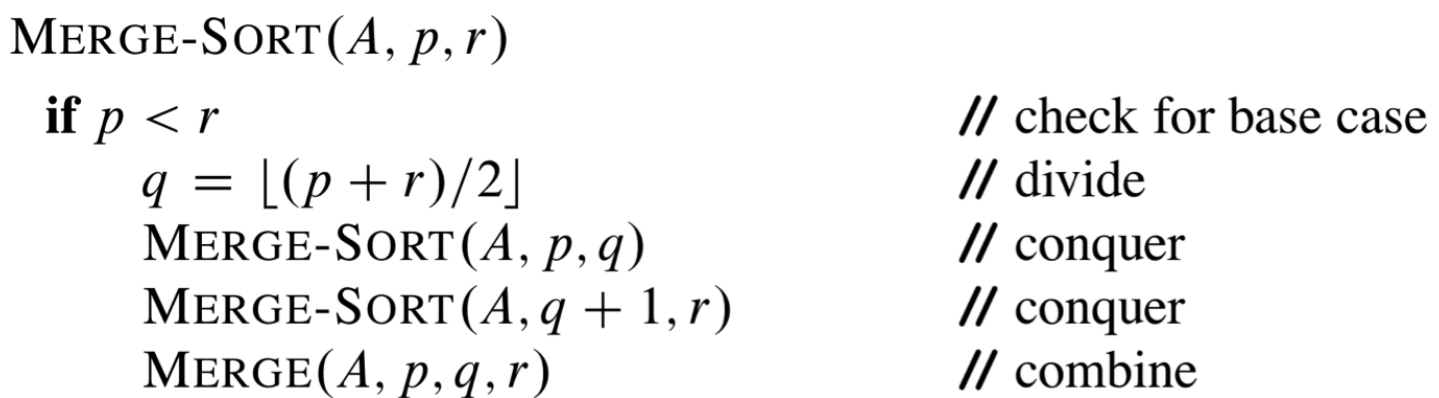
\includegraphics[width=0.7\linewidth]{images/merge-sort.png}

        \item \textbf{Merge}: Combine the two sorted subarrays into a single sorted array:
        \begin{enumerate}[noitemsep]
            \item Initializing pointers at the start of each subarray.
            \item Comparing the elements pointed to, and appending the smaller one into a new array.
            \item Advancing the pointer in the subarray from which the element was chosen.
            \item Repeating this process until all elements in both subarrays are merged into the sorted array.
 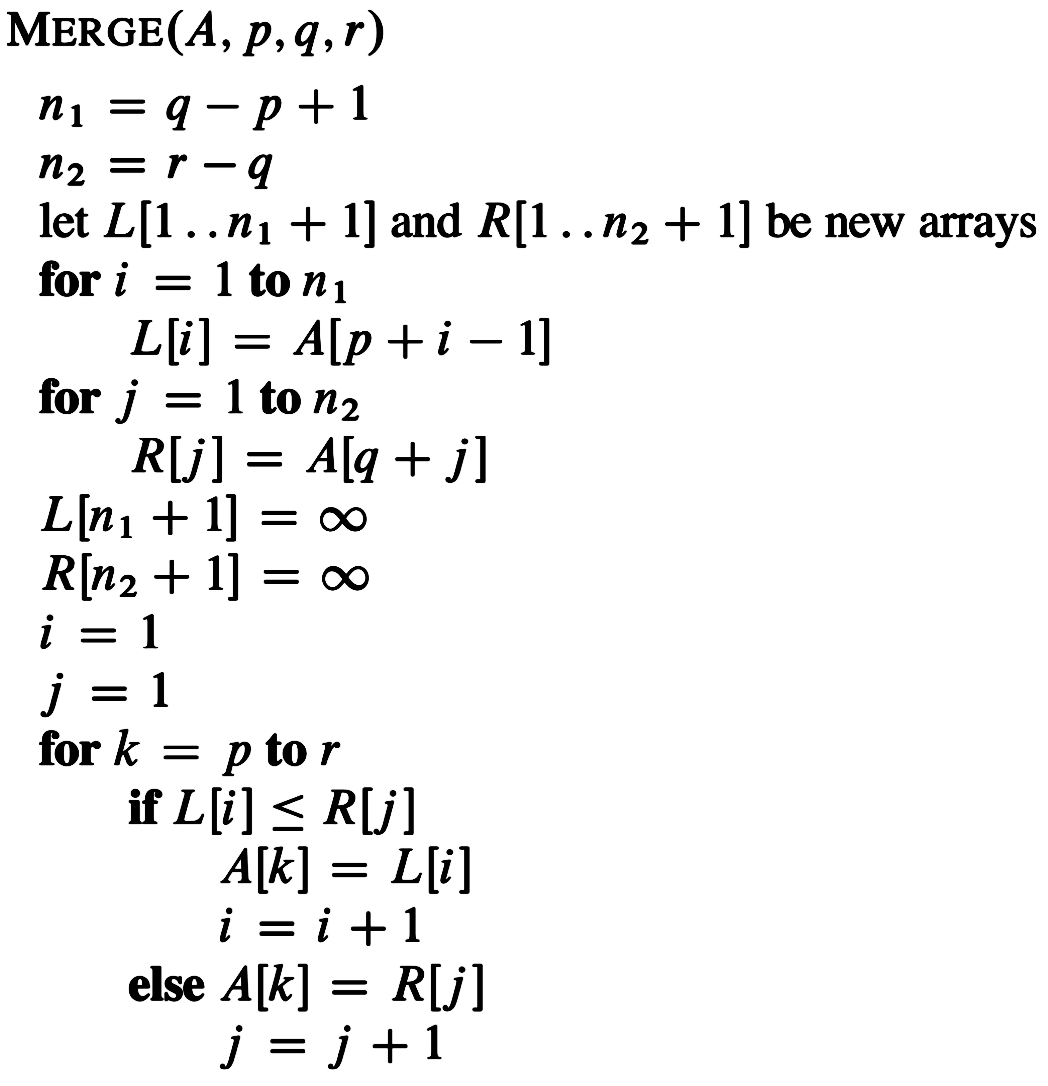
\includegraphics[width=0.6\linewidth]{images/merge.png}

        \end{enumerate}
    \end{enumerate}
    \justifying
    \textit{Merge Cost Complexity:} \(O(n)\) per merge operation.\\
    \textit{Time Complexity:} \(O(n \log n)\)\\
    \textit{Space Complexity:} \(O(n)\)
}
}\\[3px]
\fbox{
\algoblock{0.89}{\scriptsize Strassen's Matrix Multiplication \vspace{-4px}}{
    \begin{enumerate}[noitemsep]
        \scriptsize
        \item \textbf{Divide:} Partition each of \(A, B, C\) into four \(\tfrac{n}{2} \times \tfrac{n}{2}\) submatrices: \vspace{-5px}
        \[
        \begin{pmatrix}
            C_{11} & C_{12} \\
            C_{21} & C_{22}
        \end{pmatrix}
        \;=\;
        \begin{pmatrix}
            A_{11} & A_{12} \\
            A_{21} & A_{22}
        \end{pmatrix}
        \cdot
        \begin{pmatrix}
            B_{11} & B_{12} \\
            B_{21} & B_{22}
        \end{pmatrix}.
        \]
    \begin{minipage}[t]{0.45\textwidth}
        \scriptsize
        \item  \textbf{Conquer:} Compute 7 products (recursively on \(\tfrac{n}{2} \times \tfrac{n}{2}\) matrices): \vspace{-5px}
        \[
        \begin{aligned}
        M_1 &:= (A_{11} + A_{22})(B_{11} + B_{22}), \\
        M_2 &:= (A_{21} + A_{22}) \, B_{11}, \\
        M_3 &:= A_{11} \,(B_{12} - B_{22}), \\
        M_4 &:= A_{22} \,(B_{21} - B_{11}), \\
        M_5 &:= (A_{11} + A_{12}) \, B_{22}, \\
        M_6 &:= (A_{21} - A_{11}) \,(B_{11} + B_{12}), \\
        M_7 &:= (A_{12} - A_{22}) \,(B_{21} + B_{22}).
        \end{aligned}
        \]
        \end{minipage}
        \hfill
        \begin{minipage}[t]{0.45\textwidth}
        \scriptsize

        \item \textbf{Combine:} Assemble the resulting submatrices to form \(C\): \vspace{-5px}
        \[
        \begin{aligned}
        C_{11} &= M_1 + M_4 - M_5 + M_7, \\
        C_{21} &= M_2 + M_4, \\
        C_{12} &= M_3 + M_5, \\
        C_{22} &= M_1 + M_3 - M_2 + M_6.
        \end{aligned}
        \]
            \textit{Time Complexity:} \(O(n^{\log_2 7}) \approx O(n^{2.81})\)\\
    \textit{Space Complexity:} \(O(n^2)\)
        \end{minipage}
    \end{enumerate}
    \vspace{0.5ex}
    \justifying
}}
\fbox{
    \algoblock{0.89}{\scriptsize Priority Queue}{
        \scriptsize
        Maintains a dynamic set of elements with associated priority values (keys).\\
        
        \textbf{Maximum(S):} Return element of S with highest priority (return A[1], complexity $O(1)$)\\
        
        \textbf{Insert(S,x):} Insert element x into set S\\
        1. Increment the heap size\\
        2. Insert a new node in the last position in the heap, with key $-\infty$\\
        3. Increase the $-\infty$ value to key using Heap-Increase-Key\\
        
        \textbf{Extract-Max(S):} Remove and return element of S with highest priority\\
        1. Make sure heap is not empty\\
        2. Make a copy of the maximum element (the root)\\
        3. Make the last node in the tree the new root\\
        4. Re-heapify the heap, with one fewer node\\
        5. Return the copy of the maximum element\\
        
        \textbf{Increase-Key(S,x,k):} Increase the value of element x's key to the new value k\\
        1. Make sure key $\geq$ A[i]\\
        2. Update A[i]'s value to key\\
        3. Traverse the tree upward comparing new key to the parent and swapping if necessary\\
        
        \textit{Time Complexity:} Insert, Extract-Max, Increase-Key: $O(\log n)$ \quad Maximum: $O(1)$\\
        \textit{Space Complexity:} $O(n)$}}}
\begin{minipage}[t]{0.49\textwidth}
\fbox{
\algoblock{0.8}{\scriptsize Heap}{
    \scriptsize
    \fbox{
        \begin{minipage}[htp]{0.23\textwidth}
            \scriptsize
            Root is A[1] \\
            Left(i) = 2i \\ 
            Right(i) = 2i + 1\\
            Parent(i) =$\lfloor i/2 \rfloor$ \\
            \vspace{-5px}
        \end{minipage}
    } \textbf{\scriptsize Max-Heapify(heapify subtree rooted at i)} \\

    \begin{minipage}[htp]{0.55\textwidth}
        \scriptsize
        \begin{justify}
        1. Starting at the root\\
        2. Compare A[i], A[Left(i)], A[Right(i)]\\
        3. If necessary, swap A[i] with the largest of the two children to preserve heap property\\
        4. \textbf{Max-Heapify} the swapped child\\
        5. Continue this process of comparing and swapping down the heap, until subtree rooted at i is max-heap
        \end{justify}
    \end{minipage}
    \hfill
    \begin{minipage}[htp]{0.43\textwidth}
        \begin{center}
            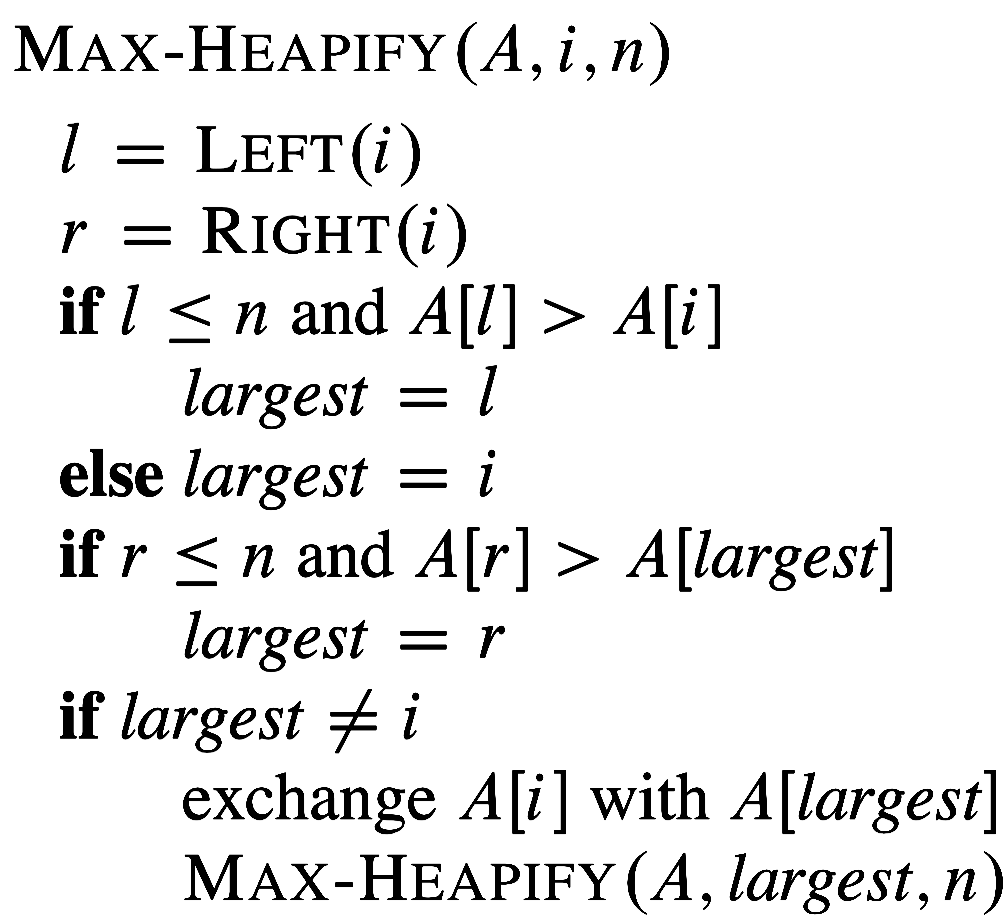
\includegraphics[width=0.9\linewidth]{images/heapify.png}
        \end{center}
    \end{minipage}\\
    \textit{Time Complexity:} \(O(\log(n))\) \quad \textit{Space Complexity:} \(O(1)\)\\
    \textbf{\scriptsize Build-Max-Heap (build a max-heap from an array)}

    \begin{minipage}[htp]{0.55\textwidth}
        \scriptsize
        1. Start from the last non-leaf node, which is located at index \(\frac{n}{2} - 1\) (in a zero-indexed array).\\
        2. Move upwards to the root (index \(0\)) and perform the following:\\
        \quad a. \textbf{Max-Heapify} the current node.\\
        \quad b. Ensure that the subtree rooted at this node satisfies the max-heap property.\\
        3. Repeat this process until the root node is processed.\\
        4. After the entire process, the array \(A\) represents a valid max heap.
    \end{minipage}
    \begin{minipage}[htp]{0.35\textwidth}
        \begin{center}
            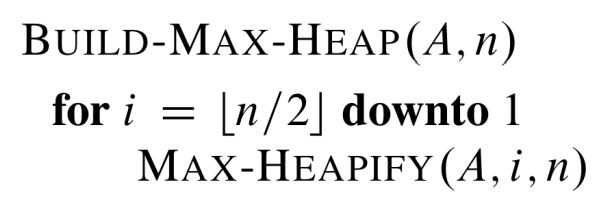
\includegraphics[width=1.2\linewidth]{images/build-max-heap.png}
        \end{center}
    \end{minipage}\\
    \textit{Time Complexity:} \(O(n)\) \quad \textit{Space Complexity:} \(O(1)\)\\
    \textbf{\scriptsize Heap Sort}\\
    \begin{minipage}[htp]{0.55\textwidth}
        \scriptsize
        \textbf{1. Build a Max Heap:}\\
        a. Convert the given array into a max heap.\\
        b. Start from the last non-leaf node and move upwards to the root, heapifying each node.\\
        c. Ensure that each parent node is greater than its child nodes.
    \end{minipage}
    \begin{minipage}[htp]{0.43\textwidth}
        \begin{center}
            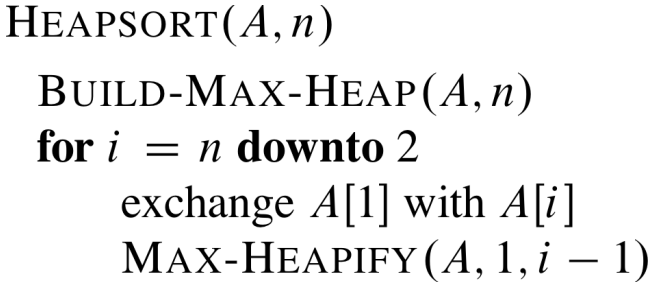
\includegraphics[width=0.9\linewidth]{images/heapsort.png}
        \end{center}
    \end{minipage}\\
    
    \textbf{2. Extract Maximum Elements:}\\
    a. Swap the root of the heap (maximum value) with the last element of the heap.\\
    b. Reduce the heap size by one to exclude the last element from the heap.\\
    c. Heapify the root element to maintain the max heap property.\\
    d. Repeat this process until the heap size becomes 1.\\

    \textbf{3. Final Sorted Array:}\\
    a. After extracting maximum elements one by one, the sorted array is obtained.\\
    b. The array is sorted in ascending order since the maximum element is placed at the end.
    
    \textit{Time Complexity:} \(O(n\,log \,n)\) \quad \textit{Space Complexity:} \(O(1)\)\\
}}
\fbox{\begin{minipage}[htp]{0.9\textwidth}
    \scriptsize
    \textbf{\scriptsize Linked List}\\
        \scriptsize
        Linear data structure where each node contains: \\
        1. \textbf{key/data}: The value stored in the node \\
        2. \textbf{next}: A pointer to the next node in the sequence \\
        3. \textbf{prev}: A pointer to the previous node (in doubly linked lists) \\
    \textbf{\scriptsize List-Search\\(find a node with a given key)}\\
    \begin{minipage}[htp]{0.45\textwidth}
        \scriptsize
        1. Start from the head of the linked list.\\
        2. Traverse the list by following the next pointers.\\
        3. Compare each node's key with the target key.\\
        4. Return the node if the key is found.\\
        5. Return NULL if the end of the list is reached without finding the key.
    \end{minipage}
    \begin{minipage}[htp]{0.45\textwidth}
        \begin{center}
            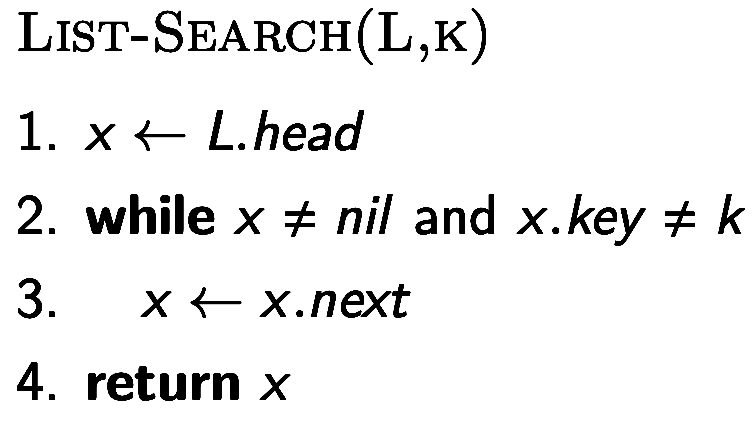
\includegraphics[width=0.95\textwidth]{images/list-search.png}
        \end{center}
    \end{minipage}\\
    \textit{Time Complexity:} \(O(n)\) \quad \textit{Space Complexity:} \(O(1)\)\\
    \textbf{\scriptsize List-Insert\\ (insert a new node at the beginning)}\\
    \begin{minipage}[htp]{0.55\textwidth}
        \scriptsize
        1. Create a new node with the given key.\\
        2. Set the next pointer of the new node to point to the current head.\\
        3. If implementing a doubly linked list, set the prev pointer of the current head to the new node.\\
        4. Update the head pointer to point to the new node.\\
        5. If the list was empty, update the tail pointer as well.
    \end{minipage}
    \begin{minipage}[htp]{0.43\textwidth}
        \begin{center}
            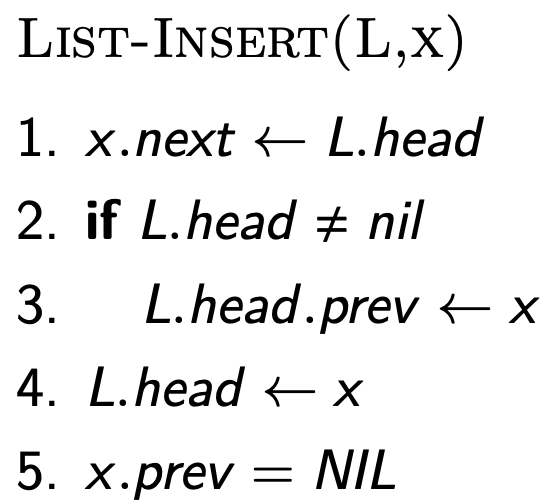
\includegraphics[width=0.75\linewidth]{images/list-insert.png}
        \end{center}
    \end{minipage}\\
    \textit{Time Complexity:} \(O(1)\) \quad \textit{Space Complexity:} \(O(1)\)\\
    \textbf{\scriptsize List-Delete \\(remove a node from the list)}\\
    \begin{minipage}[htp]{0.55\textwidth}
        \scriptsize
        1. Find the node to be deleted (may require traversal).\\
        2. If the node is the head, update the head pointer to the next node.\\
        3. Otherwise, update the next pointer of the previous node to skip the node being deleted.\\
        4. For doubly linked lists, also update the prev pointer of the next node.\\
        5. Free the memory allocated for the deleted node.\\
        6. Handle edge cases: empty list, deleting the only node, or deleting the tail.
    \end{minipage}
    \begin{minipage}[htp]{0.43\textwidth}
        \begin{center}
            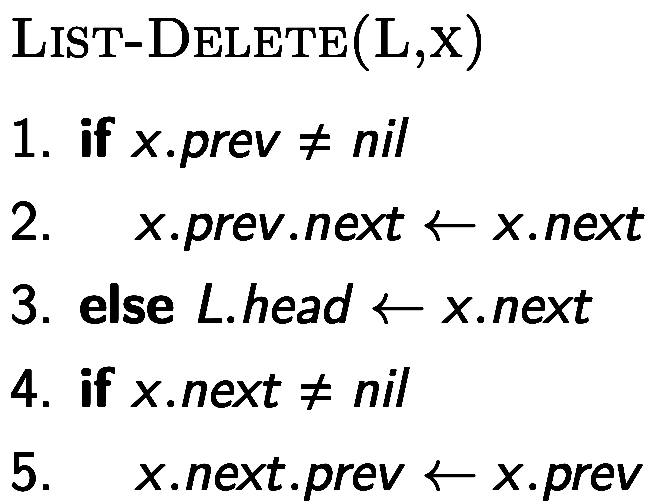
\includegraphics[width=0.75\linewidth]{images/list-delete.png}
        \end{center}
    \end{minipage}\\
    \textit{Time Complexity:} \(O(n)\) for finding the node, \(O(1)\) for deletion \\ \textit{Space Complexity:} \(O(1)\)
\end{minipage}}
\end{minipage}
\hspace{-15px}
\begin{minipage}[t]{0.49\textwidth}
\fbox{\begin{minipage}[t]{0.9\textwidth} % Changed [htp] to [t] for top alignment
    \scriptsize
    \textbf{Binary Search Trees (BST)}\\
    \textbf{Properties}\\
        \begin{itemize}
        \item[-] The left subtree of a node contains only nodes with keys less than the node's key
        \item[-] The right subtree of a node contains only nodes with keys greater than the node's key
        \item[-] Both the left and right subtrees are also binary search trees
    \end{itemize}
    \textbf{Node Structure:}\\
    Each node in a BST typically contains:
    \begin{enumerate}
        \item \textbf{key}: The value stored in the node \\
        \item \textbf{left}: A pointer to the left child \\
        \item \textbf{right}: A pointer to the right child \\
        \item \textbf{parent}: A pointer to the parent node (optional) \\
    \end{enumerate}
    
    \textbf{\scriptsize BST-Search\\(find a node with a given key)}\\
    \begin{minipage}[t]{0.45\textwidth} % Using [t] for consistency
        \scriptsize
        1. Start from the root of the tree.\\
        2. If the root is NULL, return NULL.\\
        3. If the key equals the root's key, return the root.\\
        4. If the key is less than the root's key, recursively search the left subtree.\\
        5. If the key is greater than the root's key, recursively search the right subtree.
    \end{minipage}
    \begin{minipage}[t]{0.45\textwidth} % Using [t] for consistency
        \begin{center}
            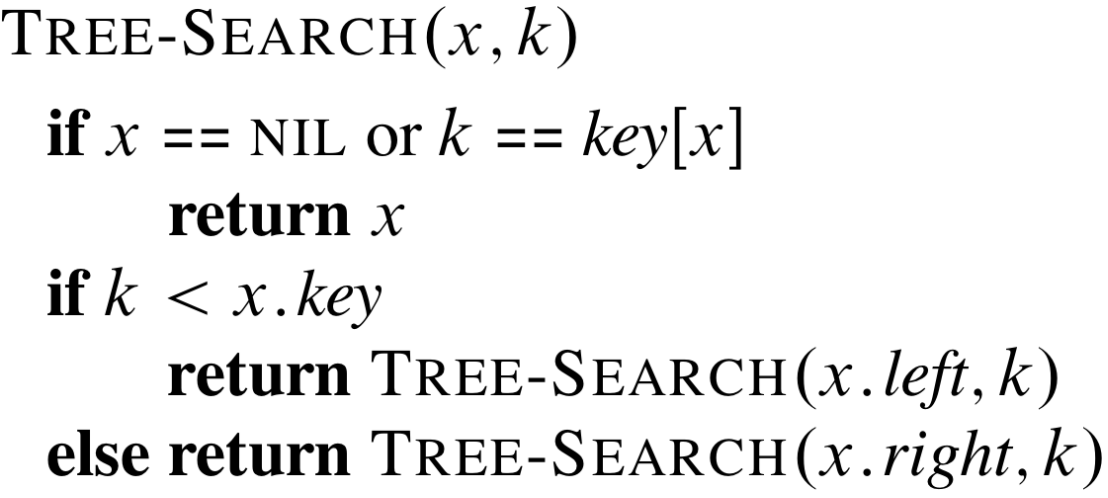
\includegraphics[width=1.1\textwidth]{images/bst-search.png}
        \end{center}
    \end{minipage}\\
    \textit{Time Complexity:} \(O(\log n)\) average, \(O(n)\) worst case \quad \textit{Space Complexity:} \(O(\log n)\) for recursion\\
    
    \textbf{\scriptsize BST-Minimum\\(find the minimum key in the tree)}\\
    \begin{minipage}[htp]{0.55\textwidth} % Using [t] for consistency
        \scriptsize
        1. Start from the root of the tree.\\
        2. If the root is NULL, return NULL.\\
        3. Traverse the tree by following the left child pointers until reaching a node with no left child.\\
        4. Return this leftmost node, which contains the minimum key.
    \end{minipage}
    \begin{minipage}[htp]{0.43\textwidth} % Using [t] for consistency
        \begin{center}
            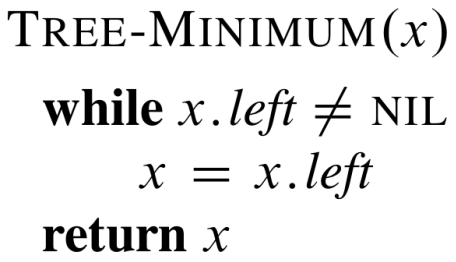
\includegraphics[width=0.65\textwidth]{images/bst-minimum.png}
        \end{center}
        \vfill
    \end{minipage}\\
    \textit{Time Complexity:} \(O(h)\) where h is the height of the tree \quad \textit{Space Complexity:} \(O(1)\)\\
    
    \textbf{\scriptsize BST-Maximum\\(find the maximum key in the tree)}\\
    \begin{minipage}[htp]{0.55\textwidth} % Using [t] for consistency
        \scriptsize
        1. Start from the root of the tree.\\
        2. If the root is NULL, return NULL.\\
        3. Traverse the tree by following the right child pointers until reaching a node with no right child.\\
        4. Return this rightmost node, which contains the maximum key.
    \end{minipage}
    \begin{minipage}[htp]{0.43\textwidth} % Using [t] for consistency
        \begin{center}
            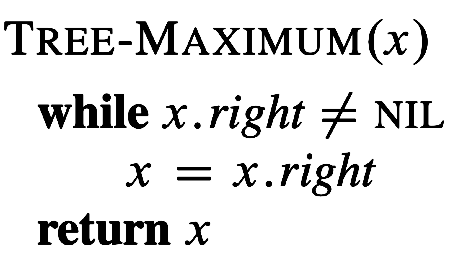
\includegraphics[width=0.75\textwidth]{images/bst-maximum.png}
        \end{center}
    \end{minipage}\\
    \textit{Time Complexity:} \(O(h)\) where h is the height of the tree \quad \textit{Space Complexity:} \(O(1)\)\\
    
    \textbf{\scriptsize BST-Successor\\(find the node with the next larger key)}\\
    \begin{minipage}[htp]{0.55\textwidth} % Using [t] for consistency
        \scriptsize
        1. If the node has a right subtree, return the minimum node in that right subtree.\\
        2. Otherwise, traverse up the tree using parent pointers.\\
        3. Find the first ancestor for which the given node is in its left subtree.\\
        4. Return this ancestor as the successor.\\
        5. If no such ancestor exists, there is no successor.
    \end{minipage}
    \begin{minipage}[htp]{0.43\textwidth} % Using [t] for consistency
        \begin{center}
            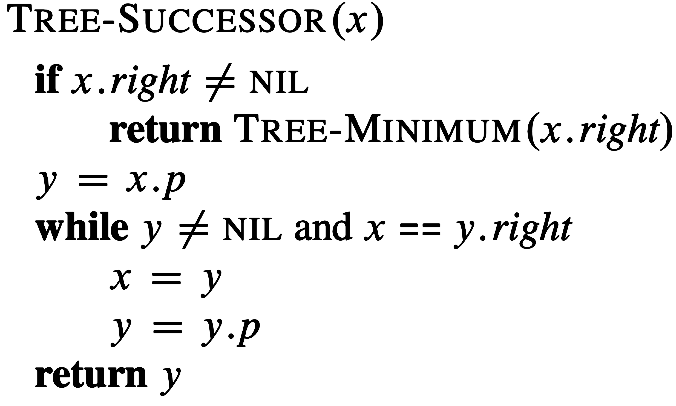
\includegraphics[width=0.9\textwidth]{images/bst-successor.png}
        \end{center}
    \end{minipage}\\
    \textit{Time Complexity:} \(O(h)\) where h is the height of the tree \quad \textit{Space Complexity:} \(O(1)\)\\
    
    \textbf{\scriptsize BST-Predecessor\\(find the node with the next smaller key)}\\
        \begin{minipage}[htp]{0.55\textwidth} % Using [t] for consistency
        \scriptsize
        1. If the node has a left subtree, return the maximum node in that left subtree.\\
        2. Otherwise, traverse up the tree using parent pointers.\\
        3. Find the first ancestor for which the given node is in its right subtree.\\
        4. Return this ancestor as the predecessor.\\
        5. If no such ancestor exists, there is no predecessor.
    \end{minipage}
    % Note: Missing image minipage for Predecessor, assuming it's intended or will be added later.
\end{minipage}}
\end{minipage}


\end{document}





